% !TEX program = xelatex
% XeLaTeX source for the 5 x 8 inch edition.
\documentclass[10pt,twoside,openany]{book}

\usepackage{geometry}
\geometry{
  paperwidth=5in,
  paperheight=8in,
  top=0.7in,
  bottom=0.7in,
  inner=0.5in,
  outer=0.5in,
  headheight=10pt,
  headsep=20pt,
  footskip=25.2pt
}
\addtolength{\textheight}{-12pt}

\usepackage{fontspec}
\usepackage{xeCJK}
\usepackage{setspace}
\defaultfontfeatures{Ligatures=TeX}
\setmainfont[Path=../fonts/]{SourceHanSerifCN-Regular.otf}
\setCJKmainfont[Path=../fonts/]{SourceHanSerifCN-Regular.otf}
\setsansfont[Path=../fonts/]{SourceHanSansCN-Medium.otf}
\setCJKsansfont[Path=../fonts/]{SourceHanSansCN-Medium.otf}
\newfontfamily\SeparatorFont{lmroman10-regular.otf}
\xeCJKsetup{PunctStyle=plain}

\usepackage{fancyhdr}
\usepackage{xcolor}
\usepackage{pdfpages}
\usepackage[unicode=true,hidelinks]{hyperref}
\definecolor{PrimaryInk}{HTML}{161618}
\definecolor{SecondaryInk}{HTML}{5C5C62}
\color{PrimaryInk}
\hypersetup{
  pdftitle={Mi novia Jing Tian},
  pdfauthor={Justin Sun},
  pdfsubject={5 x 8 inch XeLaTeX edition}
}

% Body paragraphs begin flush with the text block.
\setlength{\parindent}{0pt}
\setlength{\parskip}{0pt}
\setlength{\topskip}{10pt}
\renewcommand{\baselinestretch}{1}
\clubpenalty=10000
\widowpenalty=10000
\displaywidowpenalty=10000
\brokenpenalty=10000
\raggedbottom

\fancypagestyle{bodyrunning}{
  \fancyhf{}
  \fancyhead[LO]{\sffamily\fontsize{8}{10}\selectfont\color{SecondaryInk}Mi novia Jing Tian}
  \fancyhead[RO]{\sffamily\fontsize{8}{10}\selectfont\color{SecondaryInk}\thepage}
  \fancyhead[LE]{\sffamily\fontsize{8}{10}\selectfont\color{SecondaryInk}\thepage}
  \fancyhead[RE]{\sffamily\fontsize{8}{10}\selectfont\color{SecondaryInk}Mi novia Jing Tian}
  \renewcommand{\headrulewidth}{0pt}
  \renewcommand{\footrulewidth}{0pt}
}

\fancypagestyle{bodyopening}{
  \fancyhf{}
  \fancyfoot[C]{\sffamily\fontsize{8}{10}\selectfont\color{SecondaryInk}\thepage}
  \renewcommand{\headrulewidth}{0pt}
  \renewcommand{\footrulewidth}{0pt}
}

\newcommand{\BodySingleLeading}{17.3076923}
\newcommand{\StoryParagraph}[2]{%
  \begingroup
  \rmfamily
  \setstretch{1.3}%
  \fontsize{9.5}{\BodySingleLeading}\selectfont
  #2\par
  \vspace{#1pt}
  \endgroup
}

\newcommand{\NarrativeBreak}{%
  \par\penalty10000
  \vspace{37.4pt}
  \noindent\hbox to \textwidth{\hfil\SeparatorFont\setstretch{1.3}\fontsize{9.5}{\BodySingleLeading}\selectfont\char"002D\kern0.12em\char"002D\kern0.12em\char"002D\hfil}\par
  \vspace{31.4pt}
  \penalty10000
}

\newcommand{\UnprintedPause}{%
  \par\penalty10000\vspace{22pt}\penalty10000
}

\begin{document}
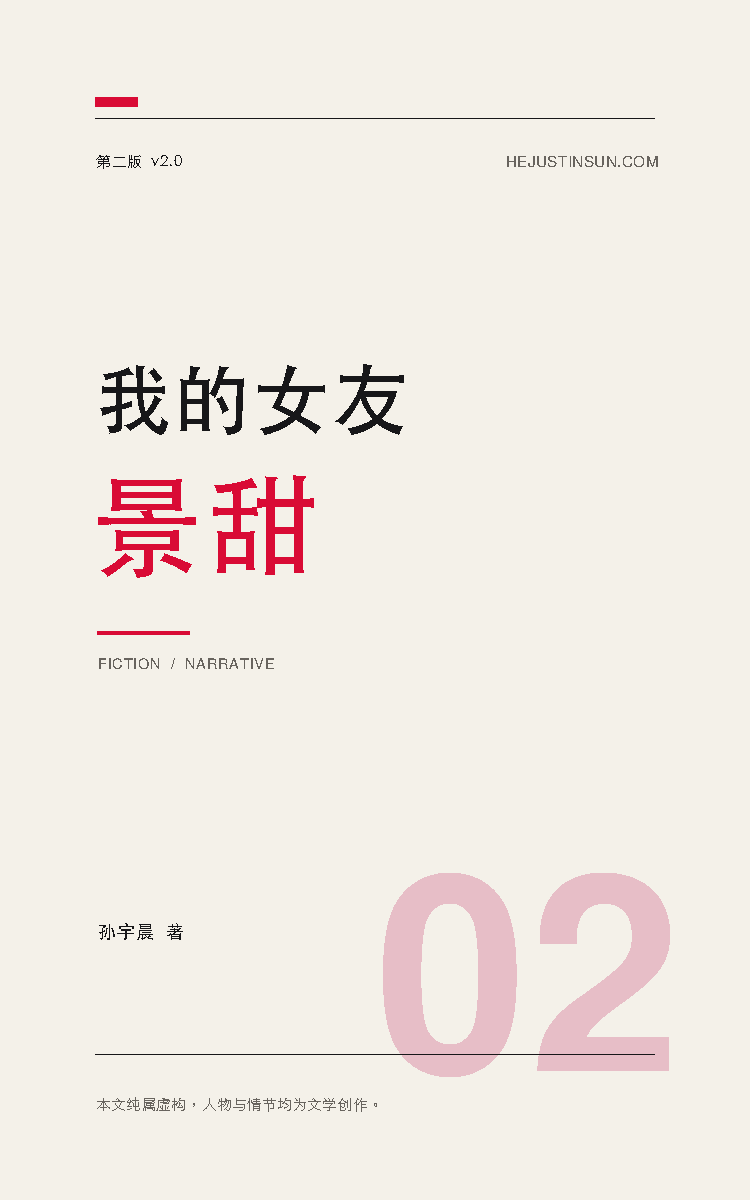
\includepdf[
  pages=1,
  fitpaper=true,
  noautoscale=true,
  pagecommand={\thispagestyle{empty}}
]{../assets/cover.pdf}

\pagenumbering{arabic}
\setcounter{page}{1}
\pagestyle{bodyrunning}
\thispagestyle{bodyopening}
% Opening-page breathing room.
\vspace*{70.817pt}

\StoryParagraph{3}{El peso de un óvulo: tres coma cinco microgramos.}

\StoryParagraph{3}{El peso de cincuenta millones de dólares en efectivo: dos toneladas y media.}

\StoryParagraph{3}{Lo que Jing Tian me pidió por teléfono desde el Montage Laguna Beach fue lo segundo. Lo que dejaba en prenda era lo primero.}

\StoryParagraph{3}{Fue allí a la extracción de óvulos. El hijo, por gestación subrogada, nacería según el cálculo en 2027; con un poco de prisa, aún caería en el año del Caballo. Lo propuso ella. Al llegar a la clínica dijo que sin los cincuenta millones no se extraía nada.}

\UnprintedPause

\StoryParagraph{0}{El Montage Laguna Beach está sobre un acantilado; abajo, el Pacífico. La planta entera reservada, treinta días, un millón de dólares, por su privacidad. Se quedó ocho días y se fue.}

\StoryParagraph{0}{Los veintidós días restantes, las limpiadoras del hotel subieron cada mañana como siempre. Me lo contó mi asistente, que se cruzó con una al ir a devolver las llaves: una mujer mexicana empujaba el carrito, entraba habitación por habitación, cambiaba las toallas, pasaba el paño por las superficies, remetía la esquina de la sábana, salía y cerraba la puerta. La planta entera, dos horas.}

\StoryParagraph{0}{La asistente le preguntó por qué seguían limpiando si no vivía nadie.}

\StoryParagraph{0}{Dijo: “En el registro figura que hay alguien”.}

\StoryParagraph{0}{Un Versalles sin reina.}

\StoryParagraph{0}{De pronto caí en la cuenta: a Jing Tian le gusta esto. A Jing Tian le gusta que un lugar esté vacío por ella. Que no pase nada.}

\StoryParagraph{3}{Vacío junto con el Montage Laguna Beach quedó también un Gulfstream G700, plantado con aire incómodo en Van Nuys, con la tripulación presentándose cada día como siempre.}

\StoryParagraph{3}{Al octavo día hizo aquella llamada. Después nadie volvió a verla.}

\NarrativeBreak

\StoryParagraph{0}{En 2007 ya había alguien quemando dinero por ella. Ese año yo acababa de entrar en la Universidad de Pekín.}

\StoryParagraph{3}{El que quemaba dinero, claro, no era yo.}

\StoryParagraph{3}{QQ hizo saltar una ventana emergente; la imagen del anuncio era ella. Fue en aquel viejo Lenovo IBM, con una resolución borrosísima. Guardé la imagen.}

\StoryParagraph{3}{Yo me conectaba desde un dormitorio de la Universidad de Pekín que costaba mil yuanes al año. La encontré en Xiaonei (el Facebook chino) y le mandé una solicitud de amistad. Xiaonei pedía escribir una frase. Escribí y borré, borré y escribí, unos cuarenta minutos. Al final mandé: “Hola”.}

\StoryParagraph{3}{No me aceptó.}

\StoryParagraph{3}{Quizá nunca llegó a usar Xiaonei.}

\StoryParagraph{3}{En todos los años que siguieron, hiciera lo que hiciera, pensaba en una sola pregunta: a qué altura me aceptaría. Lo pensé con los primeros mil millones. Lo pensé con los diez mil millones.}

\StoryParagraph{3}{Después dejé de pensarlo. Renren había cerrado hacía mucho.}

\StoryParagraph{3}{No mandé una segunda solicitud.}

\StoryParagraph{3}{En 2011 hacía frío en Pekín. Me compré un plumífero de ciento cincuenta yuanes. Recuerdo el precio porque dudé tres días.}

\StoryParagraph{3}{Ese mismo año ella rodó una película de ciento cincuenta millones de yuanes, \textit{Los Reinos Combatientes}. Sun Honglei, Francis Ng, Kim Hee-sun, Kiichi Nakai, Jiang Wu fueron traídos para hacer de comparsas, igual que diecinueve años más tarde el Montage Laguna Beach y el Gulfstream G700; no sabían qué hacían allí, pero ya que habían venido algo tendría que pasar, pero no pasó nada.}

\StoryParagraph{3}{Después vino \textit{La Gran Muralla}, de ciento cincuenta millones de dólares. Zhang Yimou, Andy Lau, Matt Damon. Después, Jackie Chan. La lista del universo Jing Tian se hacía cada vez más larga.}

\StoryParagraph{3}{Yo ya estaba entonces en Estados Unidos: estudiaba, montaba empresas, cada vez más ocupado. Lo único que no cambió: con cada aparato nuevo, por engorroso que fuera, pasaba aquella imagen de QQ.}

\StoryParagraph{3}{Diecinueve años después, la lista me añadió a mí.}

\NarrativeBreak

\StoryParagraph{3}{Nos vimos por primera vez en el Rosewood. Siempre creí que el día que la viera estaría nervioso.}

\StoryParagraph{3}{No lo estuve.}

\StoryParagraph{3}{Era más delgada que en las fotos, vestía de cualquier manera, recostada en el sofá. La miré y de pronto no pude recordar qué era exactamente lo que había estado esperando.}

\StoryParagraph{3}{La llevé a ver el plátano de Cattelan. Lo miró un buen rato y me preguntó cuánto costaba.}

\StoryParagraph{3}{Seis millones doscientos mil dólares.}

\StoryParagraph{3}{Dijo: “¿Y cuando se pudra, qué?”.}

\StoryParagraph{3}{Me quedé callado. Dijo: “Da igual. Vamos al cine”.}

\StoryParagraph{3}{Dije que sí.}

\StoryParagraph{3}{Dijo que en la sala no podía haber nadie más que nosotros dos.}

\StoryParagraph{3}{Dije que sí.}

\StoryParagraph{3}{Salí a hacer una llamada. Cuando volví, ella seguía de pie frente al plátano.}

\StoryParagraph{3}{La película era \textit{Zootopia 2}.}

\StoryParagraph{3}{Una sala de cine para dos personas: esa escena suele darse en una proyección privada para los censores.}

\StoryParagraph{3}{Hice que mi asistente comprara todas las butacas del cine.}

\StoryParagraph{3}{Había leído artículos que denunciaban la compra de taquilla falsa: entradas agotadas y solo dos espectadores. Ahora lo entendí: quizá no todo era por la taquilla.}

\StoryParagraph{3}{Comprar todas las butacas no era difícil; lo difícil eran las entradas ya vendidas. La asistente y los guardaespaldas llegaron antes a la puerta del cine y, a cada espectador con entrada, le tendían el dinero en efectivo.}

\StoryParagraph{3}{Llegó un matrimonio con un niño; el niño ya levantaba en alto sus palomitas en la puerta.}

\StoryParagraph{3}{La asistente les tendió un fajo de billetes. El niño no entendía por qué no podían entrar. Los adultos cogieron el dinero, dieron las gracias, no preguntaron nada y se fueron.}

\StoryParagraph{3}{Ese día cobraron veintiséis personas.}

\StoryParagraph{3}{Al salir del cine cambió su foto de perfil de WeChat por la de la oficial Judy Hopps.}

\StoryParagraph{3}{Por la noche le toqué las tetas con la mano. Me apartó.}

\StoryParagraph{3}{Pensé que no quería. Retiré la mano, dispuesto a decir algo.}

\StoryParagraph{3}{No dijo nada. Se incorporó, sacó del bolso una bolsita, abrió la cremallera: dentro, una hilera de cosas, como un juego de herramientas muy pequeño.}

\StoryParagraph{3}{Dijo: “Me haces daño con las uñas”.}

\StoryParagraph{3}{Me las miré. Siempre me las había cortado de cualquier manera con el cortaúñas; los bordes quedaban en punta, y normalmente no lo notaba.}

\StoryParagraph{3}{Dijo: “Ven”.}

\StoryParagraph{3}{Puso mi mano sobre su pierna y limó las uñas una a una.}

\StoryParagraph{3}{Primero la cara gruesa; al acabar, cambiaba de cara, y luego otra vez. Limaba un rato, levantaba la mano contra la luz, miraba, seguía limando.}

\StoryParagraph{3}{Pregunté cuánto había que limar.}

\StoryParagraph{3}{Dijo: “Hasta que no arañen”.}

\StoryParagraph{3}{Diez dedos. Tardó casi una hora.}

\StoryParagraph{3}{Mientras tanto me enseñó: esta cara da la forma, esta pule; con la última no se frota de un lado a otro, se va siempre en la misma dirección.}

\StoryParagraph{3}{Dije que sí.}

\StoryParagraph{3}{Cuando terminó me giró la mano, la miró, la tocó.}

\StoryParagraph{3}{Dijo: “Ya está”.}

\StoryParagraph{3}{“Toca. Donde quieras”.}

\StoryParagraph{3}{En algún momento dijo una frase. Dijo: “Si un día ya no estoy, no habrá nadie que te pula las uñas”.}

\StoryParagraph{3}{Sonreí un poco. No dije nada.}

\StoryParagraph{0}{A los tres meses de conocerla encargué un informe. Sus proyectos de todos esos años, sus socios, las participaciones de sus empresas, Jing Guoqing, Tian Xin'ai, todas las cuentas vinculadas, el piso alquilado en Pekín, el piso comprado en Shanghái, y algunas cosas más. Estuvo listo en una semana: cuarenta y tantas páginas. Había también asuntos de hombres y de mujeres; me pareció lo menos importante.}

\StoryParagraph{0}{Algunas de esas cosas ella me las contó después, y no coincidían del todo con lo que estaba escrito. No se lo dije.}

\StoryParagraph{0}{Otras cosas nunca me las contó. Yo tampoco pregunté.}

\StoryParagraph{0}{Me creo todo lo que ella dice.}

\StoryParagraph{0}{El informe lo guardé. Lo guardo todavía.}

\StoryParagraph{3}{Pero no me creo ni una sola palabra.}

\NarrativeBreak

\StoryParagraph{3}{Dijo: “En Hong Kong hay demasiada gente, me van a reconocer. Vamos a alguna parte”.}

\StoryParagraph{3}{Dije que sí.}

\StoryParagraph{3}{Señaló Tenerife en el mapa.}

\StoryParagraph{3}{Dije que sí.}

\StoryParagraph{3}{Salí a hacer una llamada; solo al volver supe que aquel lugar estaba en el Atlántico, frente a la costa noroeste de África. Al mediodía siguiente salimos treinta personas; el A330 esperaba en el aeropuerto.}

\StoryParagraph{3}{En el dormitorio del avión me preguntó: “¿Es bonito mi nombre?”.}

\StoryParagraph{3}{Dije que era bonito.}

\StoryParagraph{3}{Dijo: “El apellido de mi padre y el apellido de mi madre, juntos. ¿No es casualidad?”.}

\StoryParagraph{3}{Dije que lo recordaba desde el primer día.}

\StoryParagraph{3}{Me abrazó y dijo: “No me llames más Jing Tian. Llámame Mamá”.}

\StoryParagraph{3}{“Sí, Mamá”.}

\StoryParagraph{3}{Después de aterrizar, el comandante vino a decirme: “Jefe, al principio la isla no nos dejaba bajar. Nunca habían visto un avión privado tan grande”.}

\StoryParagraph{3}{En la isla la regla era la misma: nadie alrededor. La asistente fue a arreglarlo, nadie preguntó por qué; esta vez yo no pregunté cuánta gente era.}

\StoryParagraph{3}{El Ritz-Carlton daba de frente al Atlántico; los ventanales eran demasiado grandes. Ella no podía dormir con una hebra de luz. Las asistentes forraron la habitación entera con cinta aislante negra: fuera, claridad de pleno día; dentro, una oscuridad de celda de castigo. La cinta se despegaba con el sol; había que ponerla de nuevo cada día.}

\StoryParagraph{3}{Las asistentes eran once en total: llegaban a las seis y media de la mañana y no se iban hasta que nos dormíamos. La cinta la ponían dos chicas, una para los marcos de las ventanas, otra para los pilotos del aire acondicionado y de los enchufes; al terminar revisaban tres veces. Compraron treinta rollos de cinta y luego otros veinte. Descubrieron que la cinta puesta después de las tres de la tarde era la que antes se caía, porque a esa hora el cristal quema más, y pasaron a ponerla por la mañana. Nadie les enseñó eso; lo sacaron probando. Lo discutían entre ellas, como se discute un oficio.}

\StoryParagraph{3}{Ella sabía cómo se llamaban esas dos chicas. Yo no.}

\StoryParagraph{3}{Paramos al borde de la carretera del parque del Teide a ver la puesta de sol; la asistente bajó del coche las rosas y descorchó el champán.}

\StoryParagraph{3}{Mamá miró el mar de nubes y dijo: “Qué belleza. Aunque no tanto como los atardeceres de Delingha, en Qinghai”.}

\StoryParagraph{3}{Yo soy de Qinghai.}

\StoryParagraph{3}{No se lo dije.}

\StoryParagraph{3}{De noche subimos a la cumbre a ver las estrellas; aun con abrigos acolchados hacía frío.}

\StoryParagraph{3}{Mamá dijo: “Pide un deseo”.}

\StoryParagraph{3}{Le pregunté qué había pedido ella.}

\StoryParagraph{3}{Mamá dijo: “No te lo digo”.}

\StoryParagraph{3}{Mamá dijo: “Es precioso. Pero hace demasiado frío. ¿Vamos a las Maldivas?”.}

\StoryParagraph{3}{Dije: “Bueno”.}

\StoryParagraph{3}{Tenerife, quince grados bajo cero; las Maldivas, veintisiete. Nueve mil quinientos kilómetros en línea recta, once horas de vuelo. Pero el aeropuerto de las Maldivas era demasiado pequeño: a mitad de camino habría que cambiar nuestro avión de fuselaje ancho por uno pequeño.}

\StoryParagraph{3}{Mamá dijo: “Los aviones pequeños hacen mucho ruido. Mejor el grande”.}

\StoryParagraph{3}{En el dormitorio del avión a las Maldivas, Mamá me dijo cuál era su deseo: tener un hijo conmigo. Tenía que ser por gestación subrogada.}

\StoryParagraph{3}{Nunca le pregunté por qué. Pensé que era miedo al dolor.}

\StoryParagraph{3}{A mitad de vuelo, Mamá se incorporó de golpe a buscar el teléfono, se conectó a Starlink y dijo: “Mal asunto”.}

\StoryParagraph{3}{Le pregunté qué pasaba.}

\StoryParagraph{3}{Dijo: “Alguien quiere amenazarme. Lleva tres días preguntando y no he contestado”.}

\StoryParagraph{3}{Pregunté cuánto pedía.}

\StoryParagraph{3}{Dijo: “Tú no te metas”.}

\StoryParagraph{3}{Estuvo tecleando mucho rato: borraba y corregía, corregía y borraba. Cuando terminó, dejó el teléfono boca abajo sobre las piernas; al rato lo giró para mirarlo otra vez.}

\StoryParagraph{3}{Pregunté quién era.}

\StoryParagraph{0}{Dijo: “Uno que estuvo conmigo antes. Finanzas. Estuvo en la cárcel. Cargó con el asunto”.}

\StoryParagraph{3}{“Salió y no tenía adónde ir. Tenía que buscarme a mí”.}

\StoryParagraph{3}{Dije: “Mejor llamar a la policía y que lo detengan”.}

\StoryParagraph{3}{Me miró. “Tú no entiendes”.}

\StoryParagraph{3}{Pregunté si se lo había dado.}

\StoryParagraph{3}{Dijo que se lo había dado.}

\StoryParagraph{3}{“¿Cuánto?”.}

\StoryParagraph{3}{“Ochenta mil”.}

\StoryParagraph{3}{Dije: “¿Y para esto hacían falta tres días de pensarlo?”.}

\StoryParagraph{3}{No dijo nada.}

\StoryParagraph{3}{El resto de aquel día casi no habló. No se durmió hasta aterrizar.}

\StoryParagraph{0}{Lo primero en llegar a Soneva Jani fue la maleta de Mamá. El equipaje de treinta personas no cabía en el avión pequeño; fue en tres. Mamá tenía una sola maleta y fue en un avión aparte: dijo que no quería que se mezclara con las de los demás.}

\StoryParagraph{0}{Soneva Jani es famoso por su no news, no shoes. Mamá se quedó tranquila.}

\StoryParagraph{3}{Mayordomos del hotel, guardaespaldas, asistentes: veintiséis personas en total, más dos pilotos de dron siguiéndonos de lejos. Las asistentes volvieron a lo de la cinta: el piloto del aire acondicionado, el piloto del enchufe, una vez y otra.}

\StoryParagraph{0}{Por la noche intercambiamos nuestros ex como quien intercambia contraseñas, como una dinastía cotejando sus nombres de era. Mamá no toleraba el menor desliz, aunque Mamá tenía una palabra prohibida: al deportista no se le mencionaba.}

\StoryParagraph{0}{No lo mencioné, aunque yo sabía que el tatuaje de la espalda de Mamá se lo había hecho por el deportista.}

\StoryParagraph{3}{Quizá era demasiado grande para borrárselo.}

\StoryParagraph{0}{Dijo: “Ahora somos una familia. A mis padres les costó mucho criarme. Tienes que pagar el precio de la novia”.}

\StoryParagraph{0}{Dije que sí.}

\StoryParagraph{0}{Dio dos nombres, Jing Guoqing y Tian Xin'ai, y dos números de cuenta.}

\StoryParagraph{0}{Treinta millones, en yuanes.}

\StoryParagraph{0}{Los transferí. Aquellos dos nombres los había visto por primera vez en las cuarenta y tantas páginas.}

\StoryParagraph{3}{Al rato me pasó el teléfono para que lo viera. Tian Xin'ai había respondido una sola palabra: “Recibido”.}

\StoryParagraph{0}{Una vez Mamá dijo: “¿Sabes en qué pienso cuando te pido estas cosas?”.}

\StoryParagraph{0}{Pregunté en qué.}

\StoryParagraph{0}{Dijo: “Pienso en si alguna vez dirás que no”.}

\StoryParagraph{0}{Dije que nunca.}

\StoryParagraph{0}{Dijo: “Entonces ya no tiene gracia”.}

\StoryParagraph{3}{Pensé: ¿acaso hay algo que yo no pueda hacer?}

\StoryParagraph{0}{En los ratos de más aburrimiento estuve trasteando con aquella imagen de QQ de 2007, para pasarla al aparato nuevo. Mamá acercó la cabeza: “¿Cómo es que guardas a mis espaldas la foto de otra mujer? ¿Quién es?”.}

\StoryParagraph{0}{Me quedé callado. No dije nada.}

\StoryParagraph{0}{Le pareció que la imagen estaba demasiado borrosa y se puso a otra cosa.}

\StoryParagraph{0}{Esa noche borré la imagen.}

\StoryParagraph{3}{Al día siguiente la recuperé del teléfono viejo.}

\StoryParagraph{0}{Mamá también pasaba el teléfono sin parar. Le pregunté qué miraba.}

\StoryParagraph{0}{Dijo: “Nada. Las miserias de pelear por el primer crédito”.}

\StoryParagraph{0}{Pelear por el primer crédito: en una película solo puede haber una estrella en primer lugar. Entre el protagonista y la protagonista, también solo uno puede ir primero.}

\StoryParagraph{0}{Dije que qué aburrimiento.}

\StoryParagraph{0}{Dijo: “Sí. Lo más duro son las parejas de rodaje: entran al set cuarenta o cincuenta días, ella rueda siempre con el mismo hombre, de noche hacen el amor y de día todavía tienen que pelear por el primer crédito”.}

\StoryParagraph{0}{Dije que era inhumano.}

\StoryParagraph{0}{Dijo que sí.}

\StoryParagraph{0}{“Pero al terminar la película, no importa cuántas veces hayan hecho el amor: se hace como si no hubiera pasado nada”.}

\StoryParagraph{3}{Luego siguió mirando media hora más.}

\StoryParagraph{0}{El 2 de enero de 2026, en Soneva Jani, año nuevo, le pedí matrimonio a Mamá.}

\StoryParagraph{0}{Lo decidí la mañana del 1 de enero. El anillo estaba en Hong Kong. En la isla no había dónde comprar anillos; la asistente tomó un hidroavión a Malé y volvió por la tarde con el anillo dentro de un sobre del hotel.}

\StoryParagraph{0}{Mamá dijo: “El diamante es muy pequeño”.}

\StoryParagraph{0}{Mamá dijo: “No importa. Ya me compensarás con uno grande”.}

\StoryParagraph{0}{“Otra cosa: ¿puedes venir a Pekín?”.}

\StoryParagraph{0}{Me quedé callado.}

\StoryParagraph{0}{Creyó que yo no quería ir.}

\StoryParagraph{0}{Mamá dijo: “¿Por qué eres tan bueno conmigo?”.}

\StoryParagraph{0}{Dije: “Porque me gustas”.}

\StoryParagraph{0}{Dijo: “¿Y antes eras así con otras?”.}

\StoryParagraph{0}{Dije que no.}

\StoryParagraph{3}{Sonrió un poco. No dijo nada.}

\StoryParagraph{0}{Una mañana desperté temprano y ella no estaba en la cama.}

\StoryParagraph{0}{Salí a mirar. Estaba sentada en la terraza, de cara al mar, y el mar entero era negro. Sin luces; aún no amanecía.}

\StoryParagraph{0}{Le pregunté por qué se había levantado tan temprano.}

\StoryParagraph{0}{Dijo: “Estoy contando días”.}

\StoryParagraph{0}{Pregunté qué contaba.}

\StoryParagraph{0}{Dijo: “Vuelve a dormir”.}

\StoryParagraph{0}{Me senté un rato a su lado, sin saber qué decir. Después volví a dormirme.}

\StoryParagraph{3}{Cuando desperté otra vez, ya estaba maquillada.}

\StoryParagraph{0}{Catorce días en las Maldivas; nadie la reconoció.}

\StoryParagraph{0}{La noche del día trece, en el restaurante, se quitó las gafas de sol. Al rato se quitó también el sombrero y lo dejó en la mesa. Así estuvo sentada toda la cena. En la mesa de al lado había una pareja de ancianos alemanes; el camarero era de Sri Lanka. Nadie la miró dos veces.}

\StoryParagraph{0}{Al terminar volvió a ponerse el sombrero.}

\StoryParagraph{0}{Mamá dijo: “Volvamos”.}

\StoryParagraph{0}{Dije: “¿No decías que aún no habías estado bastante?”.}

\StoryParagraph{3}{Dijo: “Hay demasiado silencio”.}

\UnprintedPause

\StoryParagraph{0}{De vuelta en Hong Kong, Mamá conoció a mis padres.}

\StoryParagraph{0}{Esa misma noche dijo que en su casa había que preparar el encuentro de las dos familias y la boda, y repartir dinero donde hiciera falta, cuanto más mejor. Otra vez Jing Guoqing y Tian Xin'ai.}

\StoryParagraph{0}{No pregunté por qué.}

\StoryParagraph{0}{Dije que cada tarjeta tenía un límite de un millón al día.}

\StoryParagraph{0}{Mamá dijo que era demasiado lento.}

\StoryParagraph{0}{“Transfiere con cinco”.}

\StoryParagraph{0}{Cinco tarjetas, dos cuentas, transferencias por turnos. En la tercera tarjeta dudé un momento. Terminé de transferir igual.}

\StoryParagraph{3}{Mamá dijo: “Qué poca eficiencia”.}

\StoryParagraph{0}{Dije: “Para el Año Nuevo traigamos a nuestros padres a Hong Kong y lo pasamos juntos”.}

\StoryParagraph{0}{Mamá dijo: “Este año ya quedé en pasarlo en Hainan. El que viene”.}

\StoryParagraph{0}{En la Fiesta de la Primavera hubo fuegos artificiales sobre el puerto Victoria; fue un millón de personas. Ella no.}

\StoryParagraph{0}{A las tres de la madrugada llevé a mis padres de vuelta.}

\StoryParagraph{0}{La calle estaba vacía; en el semáforo en rojo no esperaba ni un coche. Aun así me detuve.}

\StoryParagraph{0}{Mamá dijo que de momento no nos veríamos: se iba enseguida a Los Ángeles a la extracción de óvulos. Antes tenía que dejar resueltos sus asuntos.}

\StoryParagraph{0}{Mamá volvió a preguntar: “¿Puedes venir a Pekín?”.}

\StoryParagraph{0}{Me quedé callado.}

\StoryParagraph{3}{No dijo qué había en Pekín. Yo no pregunté.}

\StoryParagraph{0}{Mamá dijo que en Hong Kong había que comprar un piso, a su nombre.}

\StoryParagraph{0}{Dije: “Bueno”.}

\StoryParagraph{3}{Tampoco nos vimos en San Valentín.}

\StoryParagraph{0}{Una vez, por teléfono, dijo que esa mañana le habían sacado ocho tubos de sangre.}

\StoryParagraph{0}{Dije: “¿Tanto?”.}

\StoryParagraph{0}{Dijo: “No es para tanto”.}

\StoryParagraph{0}{Dije: “Qué duro”.}

\StoryParagraph{0}{Luego hablamos de otras cosas.}

\StoryParagraph{0}{Solo después supe que esos análisis se hacen en ayunas, el segundo o el tercer día del ciclo, sin equivocarse de fecha. Aquella mañana ella debió de salir hacia las seis; el invierno de Pekín, todavía de noche. Después los controles fueron a más. Yo lo supe porque en el resumen mensual de pagos de la asistente apareció una partida nueva. La primera vez fue el año pasado, poco dinero, unos miles de yuanes. Luego salía todos los meses, a veces dos o tres apuntes. Yo aprobaba rápido: esas cantidades no exigen mirar el detalle. Solo más tarde supe que eran los análisis de sangre, el panel de seis hormonas, las ecografías, la AMH. Para ver cuánta reserva le quedaba, cuántos óvulos podían salir, si valía la pena seguir adelante.}

\StoryParagraph{0}{Todo eso se hizo en Pekín.}

\StoryParagraph{3}{No sé en qué hospital. Tampoco sé si iba sola o alguien la acompañaba.}

\StoryParagraph{0}{El 25 de febrero aterrizó en Hong Kong.}

\StoryParagraph{0}{Dijo que no iba a Los Ángeles si antes no veía el piso de Hong Kong.}

\StoryParagraph{0}{Le mandé la decena larga de pisos vistos en el último medio año. Todos le parecieron feos. De esos pisos yo no había pisado ninguno: el asistente había pasado medio año eligiéndolos uno a uno; me los mandaba y yo se los reenviaba a ella. Uno estaba en Mid-Levels; en el vídeo se veía el puerto Victoria, grabado al atardecer. En un instante la cámara tembló y recogió en la pared la sombra de quien grababa. Miré aquella sombra y pensé: quién es este hombre, cuánto habrá caminado hoy, cuántos pisos habrá visto, si sabrá para quién es este piso.}

\StoryParagraph{3}{El tiempo apremiaba; al final subió al G700 rumbo a Los Ángeles y el 28 de febrero llegó al Montage Laguna Beach.}

\NarrativeBreak

\StoryParagraph{0}{Al octavo día Mamá llamó. Allí era por la tarde; aquí, de madrugada.}

\StoryParagraph{0}{Dijo: “Cincuenta millones. De dólares”.}

\StoryParagraph{0}{Dije: “Déjame pensarlo”.}

\StoryParagraph{0}{No dijo nada. Oí que de su lado había mar.}

\StoryParagraph{0}{Al rato dijo: “Bien”.}

\StoryParagraph{0}{Colgó.}

\StoryParagraph{3}{Desde que la conozco, nunca le había dicho “Déjame pensarlo”.}

\StoryParagraph{0}{Con Claude Code, leyendo por API, repasé todos los activos en efectivo; la conclusión fue que no me afectaría en nada. Lo verifiqué otra vez. Escribí la pregunta en Claude Code. Claude dijo: “No le des esos cincuenta millones de dólares”.}

\StoryParagraph{3}{Pregunté: “¿Ya no me ama?”.}

\StoryParagraph{3}{Claude dijo: “Del amor no me ocupo y no lo entiendo. Pero no puedes darle esos cincuenta millones de dólares”.}

\StoryParagraph{3}{Nunca le había dicho que no. No por generosidad: por miedo. Miedo a la respuesta del segundo siguiente.}

\StoryParagraph{0}{Y ahora alguien lo había dicho por mí.}

\StoryParagraph{0}{Me quedé mirando esa línea mucho rato. Lo que me puso los pelos de punta no fue su inteligencia: fue que Claude no dudó ni un instante.}

\StoryParagraph{0}{No le costaba.}

\StoryParagraph{0}{Pensé entonces: esto debe de ser algo de un orden más alto. Una persona no puede ser así.}

\StoryParagraph{3}{¿Ya no me ama?}

\StoryParagraph{3}{Al día siguiente volvió a llamar.}

\StoryParagraph{3}{Mamá dijo: “El mar es muy grande”.}

\StoryParagraph{3}{Dije: “¿Ah, sí?”.}

\StoryParagraph{3}{Dijo: “Esta planta es demasiado grande, hay eco. Por la mañana vienen a limpiar y me escondo en el baño hasta que se van”.}

\StoryParagraph{3}{Dije que podía hacer que no vinieran.}

\StoryParagraph{3}{Dijo: “No hace falta”.}

\StoryParagraph{3}{Dijo: “En la clínica me preguntan cuándo llega el padre del niño”.}

\StoryParagraph{3}{Dije que podía mandar a alguien.}

\StoryParagraph{3}{Dijo: “No hace falta”.}

\StoryParagraph{3}{Luego dijo: “¿Lo has pensado ya?”.}

\StoryParagraph{3}{No dije nada. No es que estuviera pensando; no pensaba en nada. En el teléfono, de su lado había mar; del mío, el puerto Victoria. Ninguno de los dos hablaba. Conté: once segundos.}

\StoryParagraph{3}{Jing Tian dijo: “Está bien”.}

\StoryParagraph{3}{Jing Tian dijo: “Entendido”.}

\StoryParagraph{3}{Colgó.}

\StoryParagraph{3}{Después lo repasé infinitas veces: qué más dijo en esos dos días, además de los cincuenta millones. El mar es muy grande, esta planta es demasiado grande, se escondía en el baño. Eso es todo, y lo recuerdo entero, palabra por palabra. Lo que no consigo recordar es su voz: el tono con que dijo “Entendido”.}

\StoryParagraph{0}{No consigo acordarme. Después dejé de pensarlo.}

\StoryParagraph{0}{Dejé el teléfono en la mesilla, con la pantalla hacia abajo. Y entonces hice una cosa que hasta hoy no sé explicar: me puse la mano en el pecho y conté.}

\StoryParagraph{0}{El pulso era firme.}

\StoryParagraph{0}{Volví a contar: seguía firme. Sesenta y tantos por minuto, igual que siempre. Me quedé sentado, con la mano apretada contra mi propio pecho, como un médico examinando a otro.}

\StoryParagraph{3}{Pensé: así que era esto.}

\StoryParagraph{0}{El resto del día no hice nada. Me quedé en la habitación hasta que anocheció y volvió a amanecer, mirando el puerto Victoria pasar del azul al gris y del gris al negro. A las seis de la mañana, en la orilla de enfrente, las torres del centro financiero empezaron a encenderse una a una. En algún momento la asistente llamó a la puerta para preguntar por la cena. Dije que no hacía falta.}

\StoryParagraph{3}{No lloré. Estuve todo el tiempo esperando llorar.}

\NarrativeBreak

\StoryParagraph{0}{Después la asistente me pasó las cuentas; había una partida de indemnización al hotel de Tenerife. Cuando nos fuimos, la cinta se siguió poniendo unos días más: nadie les dijo que ya no hacía falta. El hotel dijo que había estado pegada demasiado tiempo, demasiadas veces; las marcas de pegamento del marco no salían y habría que cambiar el cristal entero.}

\StoryParagraph{0}{Dije que aprobado.}

\StoryParagraph{3}{Ese cristal da al Atlántico.}

\StoryParagraph{0}{En la factura, la partida de combustible del avión costaba más que la planta entera del Montage. Pregunté. El asistente dijo que el A330 está diseñado para doscientas personas y nosotros éramos solo treinta: demasiado liviano, no cuadraba el equilibrio para el despegue. Así que cada vez había que cargar combustible de más, hasta llegar al peso. Y al llegar a destino, el combustible sobrante no se podía quedar: había que soltarlo.}

\StoryParagraph{0}{Pregunté: “¿Cada vez es así?”.}

\StoryParagraph{3}{Él dijo: “Cada vez es así”.}

\StoryParagraph{0}{También llegó una caja devuelta por la clínica de Los Ángeles. Ocho días de inyecciones de estimulación ovárica, de las que van refrigeradas. Ni una abierta.}

\StoryParagraph{3}{Y el depósito de la agencia de gestación subrogada, doscientos mil dólares, no reembolsable. La gestante estaba decidida desde enero: de California, treinta y cuatro años, dos partos. En el expediente había una foto suya; no la miré. Ella estaba lista desde enero.}

\StoryParagraph{3}{Cuando Jing Tian se fue, saqué aquella foto de 2007 y la miré una vez más. Diecinueve años: los aparatos tienen cada vez más píxeles y esta imagen parece tener cada vez menos; la cara es pura mancha. La amplié y estuve mucho rato buscando en qué se diferenciaba de la de después. No encontré ni una diferencia. Porque esa foto nunca se vio bien.}

\StoryParagraph{0}{Un día me corté las uñas con el cortaúñas y, al pasar el dedo, estaban en punta.}

\StoryParagraph{0}{Me acordé de que en el cajón seguía aquello que ella dejó.}

\StoryParagraph{0}{Lo saqué y limé un par de veces. No era así. Ella había dicho que siempre en una sola dirección; olvidé cuál era la dirección.}

\StoryParagraph{0}{Lo devolví al cajón.}

\StoryParagraph{3}{Mis uñas siguen arañando.}

\StoryParagraph{0}{Una mañana el teléfono mostró un recordatorio que la asistente había programado el año pasado al ordenar la agenda: tres meses antes de la fecha prevista del parto, preparar la habitación.}

\StoryParagraph{3}{Lo borré.}

\StoryParagraph{0}{Desde que se fue, le doy vueltas a una pregunta.}

\StoryParagraph{0}{Si aquel día se lo hubiera dado, ¿se habría quedado?}

\StoryParagraph{0}{Lo pensé mucho tiempo.}

\StoryParagraph{3}{Después saqué aquel informe y volví a leerlo. Cuarenta y tantas páginas.}

\StoryParagraph{0}{Y entonces me acordé de la noche de la Fiesta de la Primavera, mirando desde la azotea los fuegos artificiales sobre el puerto Victoria.}

\StoryParagraph{0}{Un millón de personas llegó como una marea; acabaron los fuegos y el millón de personas se retiró.}

\StoryParagraph{0}{Un millón de personas.}

\StoryParagraph{0}{Cada año es igual.}

\StoryParagraph{0}{En el Hong Kong de las tres de la madrugada,}

\StoryParagraph{3}{no pasó nada.}

\end{document}
